\cut{
1. (way ahead of time) train a statistical model over the training data
2. (at inference time) coarse-grain tokenization (i.e. finding Seqsets)
3a. run the statistical model over the user data, and use the (modified) 
    viterbi algorithm to find the most likely sequences
3b. populate histograms based on the most likely sequences
3c select candidate histograms + structure, according to heuristics
3d. break down Seqsets using not just the most likely sequences
3e. recursively repeat, go to 3a.
4. apply rewriting involving blob finding to maximize the information 
   theoretic complexity score
5. print description & construct resulting tools

We'll compose this algorithm by figure and explain it with running examples 
in Section 2.
}

\section{Algorithm}\label{sec:algo}

We propose a multi-phase algorithm to attack the problem of
automatically generating tools for ad hoc data. 
The main components of
this algorithm are {\em tokenization} of raw data, 
a top-down, divide-and-conquer {\em structure discovery} procedure,
and a format {\em refinement} phase. This is similar to 
the algorithm proposed in the \learnpads{} system. 
The key difference is, instead of tokenizing the input data into 
fixed, definite tokens and using these tokens as the input to the top-down
procedure, we produce {\em all possible} token sequences for each 
data record and use all these sequences as input to the 
recursive procedure. The goal is to compute the {\em most likely}
sequence (or subsequence) for each chunk and use these sequences to predict the 
structure of the data at each level of the recursion.

\begin{figure}[t]
\begin{centercode}
(1) train a statistical model from the labeled training data;
(2) tokenize the test data into \seqset's, one \seqset{} per chunk;
(3a) if the \seqset{} of every chunk contains only 1 or 0 edges then 
      return
    else 
      find the most probable token sequence for each chunk 
(3b) construct histograms from the most probably sequences and 
    predict a top-level structure;
(3c) break down the \seqset's and assign sub-\seqset's to each 
    sub-component of the structure;
(3d) for each sub-component, recurse to (3a);
(4) apply rewriting rules to improve the overall structure;
(5) print description and generate tools.
\end{centercode}
\caption{High-level Algorithm}\label{fig:algo}
\end{figure}

Fig. \ref{fig:algo} presents this high-level algorithm. We now explain
this algorithm step-by-step with the help of {\tt yum.txt} example.

\subsection{Training models}
Well ahead of time, a statistical model is trained with
a large pool of sample data formats. Section \ref{sec:stats} has more details
on the various models we attempted in this algorithm. To train the models,
we first label the data using a set of predefined tokens. The set of tokens
used are primarily system oriented, which include
integer, float, time, date, ip address, hostname, file path, URL, 
word, id, white space and punctuations. 
A given substring may be parsed by more than one of the token
types, and we pick a token that best represent the meaning of the data.
We assume that parsing of tokens is {\em greedy}, hence
the string ``43.8'' can be parsed by sequences 
{\tt [int] [.] [int]}, {\tt [int] [.] [float]}, or {\tt [float]},
but not by {\tt [float] [.] [int]} or {\tt [float] [.] [float]},
because the token {\tt float} would parse the entire string, even though
the string ``43'' alone can be represented by a float.

\subsection{Tokenization}
At runtime, each chunk of test data is parsed into a set of all possible 
token sequences using a modified lexer. Because these sequences have
common subsequences, we organize them in a directed acyclic graph
called \seqset. Fig.\ref{fig:seqset} shows the \seqset{} after parsing 
the substring ``2.2.13-4'' from a chunk in Fig.\ref{fig:yum}. It will
form a small part of the \seqset from parsing the entire chunk.

\begin{figure}[th]
\begin{center}
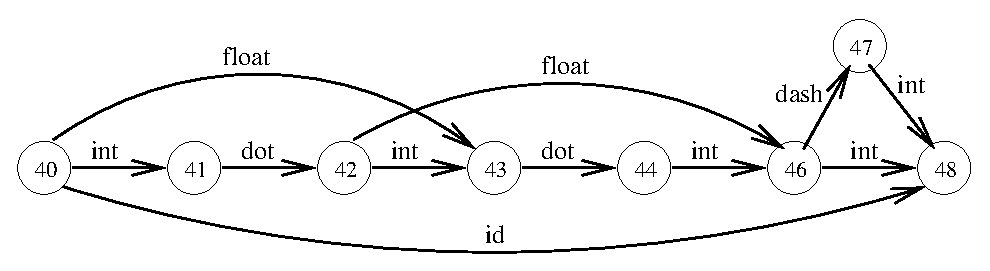
\epsfig{file=seqset.eps, width=0.9\columnwidth}
\end{center}
\caption{\seqset{} from parsing string ``2.2.13-4''}\label{fig:seqset}
\end{figure}

The edges of the \seqset{} are tokens and the vertices are the end locations
of the preceding tokens, with an exception of the leftmost vertex which
is the begin location of first character of the string.
The construction of the \seqset, though expensive, is done only once.
The \seqset{} is used as an input to the recursive structure discovery procedure
and gets updated during each recursion.

\subsection{Structure discovery}
